\documentclass[10pt]{memoir}
\setstocksize{220mm}{155mm} 	        
\settrimmedsize{220mm}{155mm}{*}	
\settypeblocksize{170mm}{116mm}{*}	
\setlrmargins{18mm}{*}{*}
\setulmargins{*}{*}{1.2}
%\setlength{\headheight}{5pt}%
\checkandfixthelayout[lines]
\linespread{1.16}
\flushbottom

%%% Hyphenation settings
\usepackage[htt]{hyphenat}
\hyphenation{he-lio-trope opos-sum}
\tracingparagraphs=1
%Hyphenation in Devanāgarī of the edition still missing? Probably this needs to be modified in babel-iast package? 

%%% babel
\usepackage[english]{babel}
\usepackage{babel-iast/babel-iast}

\babelfont[iast]{rm}[Renderer=Harfbuzz, Scale=1.3]{AdishilaSan}%AdishilaSan}
\babelfont[english]{rm}{Adobe Text Pro}

%%% more functionality
\PassOptionsToPackage{hyphens}{url}
\usepackage{hyperref}
\usepackage{pdflscape}
\usepackage{cleveref}
\usepackage{url}
\usepackage{cleveref}
\usepackage{microtype}
\usepackage{lineno}

%\usepackage{bigfoot}
%%% more functions
\usepackage[dvipsnames]{xcolor}
%\usepackage[para,perpage]{footmisc}

%%%für den Counter von Kapiteln und Sätzen! 
\newcommand{\uproman}[1]{\uppercase\expandafter{\romannumeral#1}}
\newcommand{\lowroman}[1]{\romannumeral#1\relax}

\makeindex
\newfontfamily\sanskritfont[Script=Devanagari,Mapping=RomDev,Scale=1.1]{Sanskrit2003}
\usepackage{pifont,fourier-orns,lettrine,psvectorian,paralist,enumitem,pdfpages,wrapfig,tabulary,lettrine,longtable}
\setlist[enumerate]{itemsep=0mm}
\usepackage[autostyle]{csquotes}
\usepackage[defaultlines=2,all]{nowidow}
\usepackage{ellipsis,adforn,booktabs,longtable,url,tikz}
\lineskiplimit=-3pt          

\makechapterstyle{IeT}{%
  \chapterstyle{default}
  \renewcommand*{\printchapternonum}{\centering}
  \renewcommand*{\clearforchapter}{\cleartorecto} 
  \aliaspagestyle{chapter}{empty}}
\chapterstyle{IeT}
\setsecnumdepth{none}  \openright  \nouppercaseheads
\settocdepth{subsubsection}

%%%% test better pagebreaks
%\def\fussy{%
%  \emergencystretch\z@
%  \tolerance 200%
%  \hfuzz .1\p@
%  \vfuzz\hfuzz}

%\interfootnotelinepenalty=10000\relax

%\usepackage[maxfloats=256]{morefloats}

%\maxdeadcycles=500

%raggedbottomsectiontrue
%%\checkandfixthelayout


%%%%%%%  biblatex
%\newcommand{\noun}[1]{\textsc{#1}}    %  philosophy-verbose
\usepackage[backend=biber, sorting=nyt, style=verbose]{biblatex} %%%%ORIGINAL TiE
\renewcommand*{\mkbibnamefamily}[1]{\textsc{#1}}


\DeclareFieldFormat{url}{%
  \mkbibacro{URL}\addcolon\space
  \href{#1}{\nolinkurl{\thefield{urlraw}}}}

\DeclareFieldFormat{citeurl}{%
  \href{#1}{\nolinkurl{\thefield{urlraw}}}} 


\DeclareFieldFormat{postnote}{#1}
\renewcommand{\postnotedelim}{, }
\addbibresource{bindu.bib}

%%% ekdosis
\usepackage[teiexport=tidy,parnotes=true]{ekdosis}% =tidy cleans up HTML and XML documents by fixing markup errors and upgrading legacy code to modern standards. parnotes=footnotes below or above critical apparatus

\SetLineation{lineation=page, modulo} %lineation=page sets thenumbering to start afresh at the top of each page. =modulo makes every fifth line numbered. {lineation=page} makes every line numbered! 

\renewcommand{\linenumberfont}{\selectlanguage{english}\footnotesize} %sets language of lines to English

\SetTEIxmlExport{autopar=false} %autopar=falseinstructs ekdosis to ignore blank lines in the.tex sourcefile as markers for paragraph boundaries. As a result, each paragraph of the edition must be found within an environment associated with the xml <p> element

\SetHooks{
  lemmastyle=\bfseries,
  %refnumstyle=\selectlanguage{english}\bfseries,
  refnumstyle=\selectlanguage{english}\color{blue}\bfseries,
  appheight=0.8\textheight,
}

\newif\ifinapparatus
\DeclareApparatus{source}[
%bhook=\inapparatustrue,
lang=english,
notelang=english,
% bhook=\selectlanguage{english},
bhook=\selectlanguage{english}\textbf{Sources:},%
%maxentries=4, 
%ehook=.]
%sep={] },
%nosep,
]

\newif\ifinapparatus
\DeclareApparatus{testium}[
%bhook=\inapparatustrue,
lang=english,
notelang=english,
% bhook=\selectlanguage{english},
bhook=\selectlanguage{english}\textbf{Testimonia:},
%maxentries=4, 
%ehook=.]
%nosep, 
]

% Declare \ifinapparatus and set \inapparatustrue at the beginning of
% the apparatus criticus block. Also set the language.  
\newif\ifinapparatus
  \DeclareApparatus{default}[
  %bhook=\inapparatustrue, 
  lang=english,
  %maxentries=33,
  %bhook=\selectlanguage{english},
  sep = {] },
  delim=\hskip 0.75em,
  rule=\rule{0.7in}{0.4pt},
]

\newif\ifinapparatus
\DeclareApparatus{philcomm}[
%bhook=\inapparatustrue,
lang=english,
notelang=english,
bhook=\selectlanguage{english}\textbf{Philological Commentary:},
%bhook=\selectlanguage{english},
sep={: },
]

\ekdsetup{
showpagebreaks,
spbmk = \textcolor{blue}{spb},
hpbmk = \textcolor{red}{hpb}
}

%\usepackage{fnpos}
%\makeFNmid
%\makeFNbottom
\usepackage[bottom]{footmisc}
%%%%%%%%%%%%%%%%%%%%%%%%%%%
\makeatletter
\def\blfootnote{\gdef\@thefnmark{}\@footnotetext}
\makeatother
%%%%%%%%%%%%%%%%%%%%%%%%%


% Macros and Definitions for the Print of Sigla
\def\acpc#1#2#3{{#1}\rlap{\textrm{\textsuperscript{#3}}}\textsubscript{\textrm{#2}}\space}
\def\sigl#1#2{{{#1}}\textsubscript{\textrm{#2}}}
\def\None{{\sigl{N}{1}}} \def\Noneac{\acpc{N}{1}{ac}\,} \def\Nonepc{\acpc{N}{1}{pc}\,}
\def\Ntwo{{\sigl{N}{2}}} \def\Noneac{\acpc{N}{2}{ac}\,} \def\Nonepc{\acpc{N}{2}{pc}\,}
\def\Done{{\sigl{D}{1}}} \def\Doneac{\acpc{D}{1}{ac}\,} \def\Donepc{\acpc{D}{1}{pc}\,}
\def\Dtwo{{\sigl{D}{2}}} \def\Dtwoac{\acpc{D}{2}{ac}\,} \def\Dtwopc{\acpc{D}{2}{pc}\,}
\def\Uone{{\sigl{U}{1}}} \def\Uoneac{\acpc{U}{1}{ac}\,} \def\Uonepc{\acpc{U}{1}{pc}\,}                 
\def\Utwo{{\sigl{U}{2}}} \def\Utwoac{\acpc{U}{2}{ac}\,} \def\Utwopc{\acpc{U}{2}{pc}\,}

%%%%%%%%%%%%%% Tattvabinduyoga - List of Witnesses   %%%%%%%%%%%%%%%%%%%
\DeclareWitness{ceteri}{\selectlanguage{english}cett.}{ceteri}[]   
\DeclareWitness{E}{\selectlanguage{english}E}{Printed Edition}[]    
\DeclareWitness{P}{\selectlanguage{english}P}{Pune BORI 664}[]  
\DeclareWitness{B}{\selectlanguage{english}B}{Bodleian 485}[]       
\DeclareWitness{N1}{\selectlanguage{english}N\textsubscript{1}}{NGMPP 38/31}[]
\DeclareWitness{N2}{\selectlanguage{english}N\textsubscript{2}}{NGMPP B 38/35}[]
\DeclareWitness{L}{\selectlanguage{english}L}{LALCHAND 5876}[]  
\DeclareWitness{D}{\selectlanguage{english}D}{IGNCA 30019}[] 
%\DeclareWitness{D2}{\selectlanguage{english}D\textsubscript{2}}{IGNCA 30020}[]  
\DeclareWitness{U1}{\selectlanguage{english}U\textsubscript{1}}{SORI 1574}[] 
\DeclareWitness{U2}{\selectlanguage{english}U\textsubscript{2}}{SORI 6082}[]
%%%%%%%%%%%%%% Tattvabinduyoga - Groups of Witnesses   %%%%%%%%%%%%%%%%%%%
\DeclareWitness{X}{\selectlanguage{english}\alpha}{Alpha Group: D,N1,N2,U1}[]
\DeclareWitness{Y}{\selectlanguage{english}\beta}{Beta Group: B,E,L,P,U2}[]
%%%%%%%%%%%%% Testimonia
\DeclareWitness{Ysv}{\selectlanguage{english}Ysv}{Yogasvarodaya}[] %%%add infos!  

%%%%%%%%%%%%%%%%%%%%%%%%%%%%%%%%%%%%%%%%%%%
% Macro for Editing Abbrevs.
\def\om{\textrm{\footnotesize \textit{om.}\ }} %prints om. for omitted in apparatus
\def\korr{\textrm{\footnotesize \textit{em.}\ }} %prints em. for emended in apparatus
\def\conj{\textrm{\footnotesize \textit{conj.}\ }} %prints conj. for conjectured in apparatus

% \supplied{text} EDITORIAL ADDITION -> Within \lem oder \rdg
% \surplus{text} EDITORIAL DELETION -> Within \lem oder \rdg
% \sic{text} CRUX
% \gap{text} LACUNAE -> [reason=??, unit=??, quantity=??, extent=??]


%%%%%%%%%%%%%%%%%%%%%%%%%%%%%%%%%%%%%%%%%%% All macros of this list can be used in 
% Macro for Editing Abbrevs.
\def\eyeskip{\textrm{{ab.\,oc. }}}
\def\aberratio{\textrm{{ab.\,oc. }}}
\def\ad{\textrm{{ad}}}
\def\add{\textrm{{add.\ }}}
\def\ann{\textrm{{ann.\ }}}
\def\ante{\textrm{{ante }}} 
\def\post{\textrm{{post }}}
%\def\ceteri{cett.\,}                   
\def\codd{\textrm{{codd.\ }}}

\def\coni{\textrm{{coni.\ }}}
\def\contin{\textrm{{contin.\ }}}
\def\corr{\textrm{{corr.\ }}}
\def\del{\textrm{{del.\ }}}
\def\dub{\textrm{{ dub.\ }}}

\def\expl{\textrm{{explic.\ }}} 
\def\explica t{\textrm{{explic.\ }}}
\def\fol{\textrm{{fol.\ }}}
\def\foll{\textrm{{foll.\ }}}
\def\gloss{\textrm{{glossa ad }}}
\def\ins{\textrm{{ins.\ }}}      
\def\inseruit{\textrm{{ins.\ }}} 
\def\im{{\kern-.7pt\lower-1ex\hbox{\textrm{\tiny{\emph{i.m.}}}\kern0pt}}} %\textrm{\scriptsize{i.m.\ }}}      
\def\inmargine{{\kern-.7pt\lower-.7ex\hbox{\textrm{\tiny{\emph{i.m.}}}\kern0pt}}}%\textrm{\scriptsize{i.m.\ }}}      
\def\intextu{{\kern-.7pt\lower-.95ex\hbox{\textrm{\tiny{\emph{i.t.}}}\kern0pt}}}%\textrm{\scriptsize{i.t.\ }}}           
\def\indist{\textrm{{indis.\ }}}  
\def\indis{\textrm{{indis.\ }}}
\def\iteravit{\textrm{{iter.\ }}} 
\def\iter{\textrm{{iter.\ }}}
\def\lectio{\textrm{{lect.\ }}}   
\def\lec{\textrm{{lect.\ }}}
\def\leginequit{\textrm{{l.n. }}} 
\def\legn{\textrm{{l.n. }}}
\def\illeg{\textrm{{l.n. }}}

\def\primman{\textrm{{pr.m.}}}
\def\prob{\textrm{{prob.}}}
\def\rep{\textrm{{repetitio }}}
\def\secundamanu{\textrm{\scriptsize{s.m.}}}            \def\secm{{\kern-.6pt\lower-.91ex\hbox{\textrm{\tiny{\emph{s.m.}}}\kern0pt}}}%   \textrm{\scriptsize{s.m.}}}
\def\sequentia{\textrm{{seq.\,inv.\ }}}  
\def\seqinv{\textrm{{seq.\,inv.\ }}}
\def\order{\textrm{{seq.\,inv.\ }}}
\def\supralineam{{\kern-.7pt\lower-.91ex\hbox{\textrm{\tiny{\emph{s.l.}}}\kern0pt}}} %\textrm{\scriptsize{s.l.}}}
\def\interlineam{{\kern-.7pt\lower-.91ex\hbox{\textrm{\tiny{\emph{s.l.}}}\kern0pt}}}   %\textrm{\scriptsize{s.l.}}}
\def\vl{\textrm{v.l.}}   \def\varlec{\textrm{v.l.}} \def\varialectio{\textrm{v.l.}}
\def\vide{\textrm{{cf.\ }}}
\def\cf{\textrm{{cf.\ }}} 
\def\videtur{\textrm{{vid.\,ut}}}
\def\crux{\textup{[\ldots]} }
\def\cruxx{\textup{[\ldots]}}
\def\unm{\textit{unm.}}
%%%%%%%%%%%%%%%%%%%%%%%%%%%%%%%%%%%%

% List of Scholars
\DeclareScholar{ego}{ego}[
forename=Nils Jacob,
surname=Liersch]

% Persons:14\DeclareScholar{ego}{ego}[15forename=Robert,16surname=Alessi]17% Useful shorthands:18\DeclareShorthand{codd}{codd.}{V,I,R,H}19\DeclareShorthand{edd}{edd.}{Lit,Erm,Sm}20\DeclareShorthand{egoscr}{\emph{scripsi}}{ego}

%Useful shorthands:
%\DeclareShorthand{codd}{codd.}{V,I,R,H}
%\DeclareShorthand{edd}{edd.}{Lit,Erm,Sm}
\DeclareShorthand{egoscr}{em.}{ego}
\DeclareShorthand{egoscrconj}{conj.}{ego}
\DeclareShorthand{egomute}{\unskip}{ego}

\usepackage{xparse}

\NewDocumentEnvironment{tlg}{O{}O{}}{\setlength{\leftskip}{0pt}\vspace{-1ex}\begin{quotation}}{\hfill #1\ \vspace{-1ex}\end{quotation}\vspace{-1ex}} %verse environment
%\NewDocumentEnvironment{tlg}{O{}O{}}{\begin{verse}}{॥#1\hskip-4pt ॥\\ \end{verse}}
\NewDocumentCommand{\tl}{m}{{\selectlanguage{iast} #1}}

\NewDocumentCommand{\extra}{m}{{\textcolor{gray}{#1}}} %command for additions to U2
\NewDocumentCommand{\crazy}{m}{{\textcolor{red}{#1}}} %totally corrupted passage
\NewDocumentCommand{\coro}{m}{{\textcolor{violet}{#1}}} %colour for sentence counter! 

\NewDocumentEnvironment{prose}{O{}}{\begin{otherlanguage}{iast}}{\end{otherlanguage}}
% \NewDocumentEnvironment{padd}{O{}}{\begin{otherlanguage}{iast}}{\end{otherlanguage}}
\NewDocumentEnvironment{tlate}{O{}}
%\NewDocumentEnvironment{tadd}{O{}}

%Define two commands: \skp ("sanskrit plus"), to be ignored by TeX in
%the edition text, but processed in the TEI output. Conversely, \skm
%("sanskrit minus") is to be processed in the edition text, but
%ignored if found in the apparatus criticus and in the TEI output:

\NewDocumentCommand{\skp}{m}{}
\TeXtoTEIPat{\skp {#1}}{#1}

%\NewDocumentCommand{\skpp}{m}{}
%\TeXtoTEIPat{\skpp {#1}}{#1}

\NewDocumentCommand{\skm}{m}{\unless\ifinapparatus#1-\fi}
\TeXtoTEIPat{\skm {#1}}{}

% \NewDocumentCommand{\dd}{}{/\hskip-4pt/}
\NewDocumentCommand{\dd}{}{\mbox{/\hskip-4pt/}}
\TeXtoTEIPat{\dd {}}{//}


%%% modify environments and commands
%%% TEI mapping
\TeXtoTEIPat{\begin {tlg}}{<lg>} %lg=(Group of verse (s)) contains one or more verses or lines of verse that together form a formal unit (e.g. stanza, chorus).
\TeXtoTEIPat{\end {tlg}}{</lg>}

\TeXtoTEIPat{\begin {prose}}{<p>}
\TeXtoTEIPat{\end {prose}}{</p>}

\TeXtoTEIPat{\begin {tlate}}{<p>}
\TeXtoTEIPat{\end {tlate}}{</p>}

\TeXtoTEIPat{\\}{}
\TeXtoTEIPat{\linebreak}{<br/>}
\TeXtoTEIPat{\noindent}{}
%\TeXtoTEI{tl}{l}
\TeXtoTEI{emph}{hi}
\TeXtoTEI{bigskip}{}
\TeXtoTEI{None}{N1}
\TeXtoTEI{Ntwo}{N2}
\TeXtoTEI{Done}{D1}
\TeXtoTEI{Dtwo}{D2}
\TeXtoTEI{Uone}{U1}
\TeXtoTEI{Utwo}{U2}
%\TeXtoTEIPat{/}{ |}
%\TeXtoTEI{//}{ ||}
\TeXtoTEIPat{\korr}{em. }
\TeXtoTEIPat{\conj}{conj.}
\TeXtoTEIPat{\om}{om.}
\TeXtoTEIPat{english}{}
\TeXtoTEIPat{\hskip}{}
\TeXtoTEIPat{\hskip-4pt}{}
\TeXtoTEIPat{\hskip-2pt}{}
\TeXtoTEIPat{-}{ }
\TeXtoTEIPat{4pt}{}
\TeXtoTEIPat{2pt}{}
\TeXtoTEIPat{\textcolor {#1}{#2}}{<hi rend="#1">#2</hi>} 

% Nullify \selectlanguage in TEI as it has been used in
% \DeclareWitness but should be ignored in TEI.
\TeXtoTEI{selectlanguage}{}



\FormatDiv{1}{\begin{center}\Large}{\end{center}}
\FormatDiv{2}{\begin{center}\small}{\end{center}}
\FormatDiv{3}{\bfseries}{.}
\title{Yogatattvabindu of Rāmacandra\\ A Critical Edition and Annotated Translation}
\date{\today}

\parindent=15pt
\begin{document}

% Zitiermöglichkeiten:
%\footcite[See][p.\,1]{goldstein01:_tibet_englis_diction_moder_tibet}
%\footnote{\cite{goldstein01:_tibet_englis_diction_moder_tibet}.}

\frontmatter
\thispagestyle{empty}
\begin{center}
  {\Large \emph{The Yogatattvabindu}}\\[3mm]
\end{center}



\newpage

\

\thispagestyle{empty}



\normalsize


\newpage


\begin{center}
\thispagestyle{empty}

\

\vskip 2mm

\begin{otherlanguage}{iast}
\LARGE \sanskritfont{Yogatattvabindu}
\end{otherlanguage}

\vskip .4cm

\Huge Yogatattvabindu \\[7mm]
\Large Critical Edition\\
with annotated Translation


\large

\vspace{3cm}

Von

Nils Jacob Liersch
\small
\vfill

\vfill

Indica et Tibetica Verlag \\ % $\cdot$ 
Marburg 2024

\vskip 6mm

\end{center}

\newpage
\newpage \ \thispagestyle{empty}
\small  \

\noindent

\
\vfill


\small
\noindent \textbf{Bibliographische Information Der Deutschen Bibliothek}

\noindent
Die Deutsche Bibliothek verzeichnet diese Publikation in der Deutschen Nationalbibliographie;
detaillierte bibliographische Informationen sind im Internet über http://dnb.ddb.de abrufbar.

\noindent
\textbf{Bibliographic information published by Die Deutschen Bibliothek}

\noindent
Die Deutsche Bibliothek lists this publication in the Deutsche Nationalbibliographie; detailed
bibliographic data is available in the Internet at http://dnb.ddb.de.  


\vskip 1cm

\noindent
\copyright\ Indica et Tibetica Verlag, Marburg 2024

\medskip

\noindent
Alle Rechte vorbehalten / All rights reserved

\medskip

\noindent
Ohne ausdrückliche Genehmigung des Verlages ist es nicht gestattet, das Werk oder einzelne Teile
daraus nachzudrucken, zu vervielfältigen oder auf Datenträger zu speichern.

\smallskip

\noindent
Apart from any fair dealing for the purpose of private study, research, criticism or review, no
part of this book may be reproduced or translated in any form, by print, photo form, microfilm, or
any other means without written permission. Enquiries should be made to the publishers.

\bigskip

\noindent
Satz: \ \ Nils Jacob Liersch \\
Herstellung: \ \ BoD – Books on Demand GmbH, Norderstedt  \\

\bigskip

\noindent
%\ISBN     

\normalsize

\newpage

%\maketitle
\clearpage
\tableofcontents
\addtocounter{page}{-1}
\thispagestyle{empty}
\clearpage


\mainmatter

\chapter{Conventions in the Critical Apparatus}
\section{Sigla in the Critical Apparatus}

\begin{itemize}
\item E : Printed Edition
\item P : Pune BORI 664
\item L : Lalchand Research Library LRL5876
\item B : Bodleian Oxford D 4587
\item \None : NGMPP B 38-31
\item \Ntwo : NGMPP B 38-35 / A 1327-14
\item \Done : IGNCA 30019
\item \Uone : SORI 1574
\item \Utwo: SORI 6082
\end{itemize}

\chapter{Critical Edition \& Annotated Translation}
\cleardoublepage
\begin{alignment}[
  texts=edition[class="edition"];
  translation[class="translation"],
  ]
  \begin{edition}
    \begin{prose}[p12_02]
      \noindent
%------------------------------
%asyāḥ kalāyā   dhyānayogāt    sādhakasya manasi duḥkhaṃ na bhavati / \E
%asyāḥ kalādhyānayogāt         sādhakasya manasi duḥkhaṃ na bhavati / \P
%asyāḥ kalāyāḥ  dhyānakaraṇāt  sādhakasya manasi duḥkhaṃ na bhavati / N1
%asyā kalāyā    dhyānakaraṇāt  sādhaka----manasi duḥkhaṃ na bhavati / N2
%asyāḥ kalāyāḥ  dhyānakaraṇāt  sādhakasya manasi duḥkhaṃ na bhavati / D
%
%asyāḥ kalāyā   dhyānayogāt    sādhakasya manasi duḥkhaṃ bhavati /B
%asyāḥ kalāyā   dhyānayogāt    sādhakasya manasi duḥkhaṃ bhavati /L
%asyāḥ kalāyā   dhyānakaraṇāt/ sādhakasya manasi duḥkhaṃ na bhavati / U1
%asyā  kalāyāḥ  dhyānayogāt//  sādhakasya manasi duḥkhaṃ na bhavati // \U2
%atrastāne 'haṃ devatā// sohaṃ śaktiḥ// ātmāṛṣiḥ// mokṣamārhaḥ// haṃ bhrahmordhaṃ// haṃ cakra iti// agnicakre sakaro bhavatī// prāṇīrūḍho bhave jjīva ārohaty avarohati bhavaguhāsthānaṃ pitavarṇaṃ// koṭisūryapratikāśaṃ tejaḥ sadoditaprabhā śīvodevatā// mūlamāyā śaktiḥ// hara ātmālayāvsthā dhvanisthirānādātmako khaṃḍa 'dhvani// adhorāmudrā// mūlamāyā// prakṛtidehaḥ// vāṅmanogocaraḥ// niḥprapaṃcaḥ// niḥsaṃśayaḥ// nistaraṃganirlepalakṣaṃ laya// dhyānasamādhi 
%---------------------
%asyāḥ kalāyā dhyānakaraṇāt\varc{\emend kalāyāḥ dhyānakaraṇāt \nepal \dehlia}{kalāyā dhyānayogāt \nepal \dehlia kalādhyānayogāt \pune} sādhakasya manasi duḥkhaṃ na\varc{na \edprint \pune \nepal \dehlia}{\om \oxford \lalchand} bhavati /
%Due meditation upon the digit suffering does not arise in the mind of the practitioner. 
%------------------------------
\app{\lem[wit={ceteri}]{asyāḥ}
  \rdg[wit={N2,U2}]{asyā}}
\app{\lem[wit={N2,U1}]{kalāyā}
  \rdg[wit={D,N1}]{kalāyāḥ}
  \rdg[wit={B,E,L}]{kalāyā}
  \rdg[wit={U2}]{kalāyāḥ}
  \rdg[wit={P}]{\om}}
dhyāna\app{\lem[wit={X}, alt={°karaṇāt}]{karaṇā\skp{t-sā}}
  \rdg[wit={Y}]{°yogāt}
}\app{\lem[wit={ceteri}, alt={sādhakasya}]{\skm{t-sā}dhakasya}
  \rdg[wit={N2}]{sādhaka°}}
duḥkhaṃ
manasi
\app{\lem[wit={ceteri}]{na}
  \rdg[wit={B,L}]{\om}}
bhavati/
\extra{atra
   \app{\lem[type=emendation, resp=egoscr]{sthāne}
    \rdg[wit={U2}]{stāne}}'haṃ devatā\dd{}
  so'haṃ śaktiḥ\dd{}
  ātmā ṛṣiḥ\dd{}
  mokṣamārgaḥ\dd{}
  haṃ brahmordhaṃ\dd{}
  haṃ cakra iti\dd{}
   agnicakre
   \app{\lem[type=emendation, resp=egoscr]{sakāro}
     \rdg[wit={U2}]{sakaro}}
   \app{\lem[type=emendation, resp=egoscr]{bhavati}
     \rdg[wit={U2}]{bhavatī}}\dd{}
   prāṇī rūḍho bhave:\\j-jīva ārohaty-avarohati\dd{}
bhavaguhā sthānam\dd{}
   pītavarṇam\dd{}
   koṭisūryapratikāśaṃ tejaḥ\dd{}
   sadoditaprabhā\dd{}
   \app{\lem[type=emendation, resp=egoscr]{śivo}
     \rdg[wit={U2}]{śīvo}} 
   devatā\dd{}
  mūlamāyā śaktiḥ\dd{}
  hara ātmālayāvasthā dhvanisthirā nādātmako\app{\lem[type=emendation, resp=egoscr]{'khaṇḍadhvaniḥ}
     \rdg[wit={U2}]{khaṃḍadhvani}}\dd{} 
   aghorā mudrā\dd{}
   \begin{otherlanguage}{english}\textbf{\Large{\sic*{}}}\end{otherlanguage}mūlamāyā\dd{}\begin{otherlanguage}{english}\textbf{\Large{\sic*{}}}\end{otherlanguage}\dd{}
   prakṛtidehaḥ\dd{}
   vāṅmano'gocaraḥ\dd{} %%
   niḥprapañcaḥ\dd{}
   niḥsaṃśayaḥ\dd{}
\begin{otherlanguage}{english}\textbf{\Large{\sic*{}}}\end{otherlanguage}nistaraṅganirlepalakṣaṃ %%%see pw Vol. 3, S. 229 for nistaranga
   layadhyānasamādhi\dd{}\begin{otherlanguage}{english}\textbf{\Large{\sic*{}}}\end{otherlanguage}}
    \end{prose}
  \end{edition}
  \begin{translation}
    \begin{tlate}[p12_02]
      \noindent
      \begin{euber}[f12_1]\blfootnote{\hspace{-2.2em}feet, generative organ, navel, heart, throat, uvula, middle of the eyebrows, forehead and the crown of the head.'' In the \citetitle{goraksapaddhati} 2.75-76 one finds nine places as \textit{dhyānasthāna}s, ``places for meditation'': (\textit{gudaṃ meḍhraṃ ca nābhiś ca hṛtpadmaṃ ca tad ūrdhvataḥ | ghaṇṭikā laṃbikāsthāna bhrūmadhye ca nabhobilam} || 75 || \textit{kathitāni navaitāni dhyānasthānāni yogibhiḥ | upādhitatvamuktāni kurvanty aṣṭaguṇodayam} || 76 ||) ``Anus and generative organ and navel, heart and [the place] above [the heart], uvula, tongue, middle of eyebrows and crown of the head. These are the nine places of meditation [taught] by the yogis, which free one from the limitations of the material world and bestow the eight supernatural powers.''}\end{euber}
 Due meditation upon the digit suffering does not arise in the mind of the practitioner. 
 \extra{Here, at this location the deity is ``I''(\textit{aham}). The power is the  ``he is I'' (\textit{so'ham}). The Ṛṣi is the self. The path is the liberation. Above Brahma[randhra?]\footnote{It is not clear if this \textit{brahmordhvam} signifies Brahman, Brahmā or even the \textit{brahmarandhra} \textit{cakra}. Since the syllable ``\textit{sa}'' is situated in the \textit{agnicakra} this location here could point at the upper part of the body, the point up to which the \textit{haṃ}-part of the breath ascends on inhalation.} is \textit{haṃ}\footnote{Probably the syllable ``\textit{haṃ}'' in this context refers to the first of the two syllables of the word \textit{haṃsa}.}. \textit{haṃ} is in the \textit{cakra}\footnote{This particular \textit{cakra} must refer to the current \textit{cakra} which is described here, which appears to be the exact topmost point to which the breath ascends.}. In the \textit{cakra} of fire\footnote{Since the bodily fire in most texts of yoga is situated in the navel area, the \textit{agnicakra} perhaps refers to the lowest point of the body the breath decends to.} is the letter ``\textit{sa}''. The breathing becomes developed [and] the soul ascends and descends. The place is the hiding place of existance. The colour is yellow. The spleandour is the shine of ten million suns. The shine always arises. The deity is Śiva. The power is primordial illusion. The state is the dissolution of the self into Hara\footnote{Epiphet of Śiva. Cf. for example \citetitle{hathatattvakaumudi} 25.6.} which is the unbroken sound that is not subject to sonic change having the nature of subtle sonic matter.\footnote{The term \textit{nāda} in śaivaite contexts can be taken as ``subtle sonic matter'', cf. \citetitle{tantrika3}, p. 277.} The seal is Aghorā. \textbf{\Large{\sic*{}}}Primordial illusion.\textbf{\Large{\sic*{}}}\footnote{Possibly a dittography of the mention of \textit{mūlamāyā} a few lines above. The point of mentioning it here is not clear to me.} The body is original matter. [It is] not in range of mind and speech. [It is] without manifestation. [It is] without doubt. \textbf{\Large{\sic*{}}}Absorption into meditation and dissolution is the goal without waves [and] without tarnish.\textbf{\Large{\sic*{}}}}\footnote{The meaning of the passage could not be reconstructed and translated with certainty. This is therefore to be understood as a provisional translation. The compound \textit{layadhyānasamādhi} seems to be a \textit{dvandvā}-compund of the collective unit of the three related terms. The compund could, however, also be dissolved as a \textit{tatpuruṣa} and translated as ``absorption into meditation and dissolution'', which seems to provide better sense.}
\flushpage 
      \end{tlate}
    \end{translation}
\end{alignment}
\pagebreak % after pp. 27-28
%%%%%%%%%%%%%%%%%%%%%%%%%%%%%%%%%%%%%%%%%%
%%%%%%%%%%%%%%%%%%%%%%%%%%%%%%%%%%%%%%%%%% 
%%%%%%%%PAGEBREAK%%%%%%%PAGEBREAK%%%%%%%%%
%%%%%%%%%%%%%%%%%%%%%%%%%%%%%%%%%%%%%%%%%% 
%%%%%%%%%%%%%%%%PAGEBREAK%%%%%%%%%%%%%%%%%
%%%%%%%%%%%%%%%%%%%%%%%%%%%%%%%%%%%%%%%%%% 
%%%%%%%%PAGEBREAK%%%%%%%PAGEBREAK%%%%%%%%%
%%%%%%%%%%%%%%%%%%%%%%%%%%%%%%%%%%%%%%%%%% 
%%%%%%%%%%%%%%%%%%%%%%%%%%%%%%%%%%%%%%%%%% 
%%%%%%%%%%%%%%%%%%%%%%%%%%%%%%%%%%%%%%%%%% 
%%%%%%%%%%%%%%%%%%%%%%%%%%%%%%%%%%%%%%%%%% 
%%%%%%%%PAGEBREAK%%%%%%%PAGEBREAK%%%%%%%%%
%%%%%%%%%%%%%%%%%%%%%%%%%%%%%%%%%%%%%%%%%% 
%%%%%%%%%%%%%%%%PAGEBREAK%%%%%%%%%%%%%%%%%
%%%%%%%%%%%%%%%%%%%%%%%%%%%%%%%%%%%%%%%%%% 
%%%%%%%%PAGEBREAK%%%%%%%PAGEBREAK%%%%%%%%%
%%%%%%%%%%%%%%%%%%%%%%%%%%%%%%%%%%%%%%%%%% 
%%%%%%%%%%%%%%%%%%%%%%%%%%%%%%%%%%%%%%%%%% 
%%%%%%%%%%%%%%%%%%%%%%%%%%%%%%%%%%%%%%%%%% 
%%%%%%%%%%%%%%%%%%%%%%%%%%%%%%%%%%%%%%%%%% 
%%%%%%%%PAGEBREAK%%%%%%%PAGEBREAK%%%%%%%%%
%%%%%%%%%%%%%%%%%%%%%%%%%%%%%%%%%%%%%%%%%% 
%%%%%%%%%%%%%%%%PAGEBREAK%%%%%%%%%%%%%%%%%
%%%%%%%%%%%%%%%%%%%%%%%%%%%%%%%%%%%%%%%%%% 
%%%%%%%%PAGEBREAK%%%%%%%PAGEBREAK%%%%%%%%%
%%%%%%%%%%%%%%%%%%%%%%%%%%%%%%%%%%%%%%%%%% 
%%%%%%%%%%%%%%%%%%%%%%%%%%%%%%%%%%%%%%%%%% 
\begin{alignment}[
  texts=edition[class="edition"];
  translation[class="translation"],
  ]
  \begin{edition}
    \begin{prose}[p12_03]
      \noindent
 \note[type=source, labelb=106, labele=_107e, nosep]{cf. YSv (PT p. 833): anantaparamānandasthānaṃ jñeyaṃ tadūrddhvataḥ (\textit{tadarddhataḥ} YK 1.278) | ūrddhvagatakalā tatra tasya dhyānād bhaved iti | iti siddhirājayogaṃ strīṇāṃ bhogaṃ mahāsukham | gītavādyavinodādi saśivaṃ varddhate kṣitau | dhyānaṃ nirantarañ cāsya puṇyapāpe sthire (\textit{sthirau } YK 1.280) na hi | nijarūpasya dṛṣṭiḥ syād dūrasyārthañ ca paśyati |}
 \note[type=source, labelb=106, labele=_107e, nosep]{cf. SSP 2.9 (Ed p. 32): navamam ākāśacakraṃ ṣodaśadalakamalam ūrdhvamukham | tanmadhye karṇikāyāṃ trikūṭākārāṃ \textbf{tadūrdhvaśaktiṃ} tāṃ paramaśūnyāṃ dhyāyet | tatraiva pūrṇagiripīṭhaṃ sarveṣṭasiddhipradaṃ bhavati |}
  \note[type=testium, labelb=106, labele=_107e, nosep]{cf. \citetitle{saubhagya}: navamamākāśacakram | tatra ṣoḍaśadalapadmamūrdhvamukhaṃ tanmadhyakarṇikātrikūṭākāram | tanmadhye ūrdhvaśaktiḥ | tāṃ paśyandhyāyet | tatraiva pūrṇagiripīṭhaṃ sarvecchāsiddhisādhanaṃ bhavati |}
%---------------------
%tadupari anaṃtaparamānandasya sthānam / \E
%tadupari anaṃtaparamānandasya sthānaṃ   \P
%tadupari anantaparamānaṃdasya sthānam / \N1
%tadupari anantaparamānaṃdasya sthānam / \N2
%tadupari anantaparamānaṃdasya sthānaṃ / \D
%tadupari anantaparamānaṃdasya sthānam vartate/ \B
%tadupari anaṃtaparamānaṃdasya sthānam vartate/ \L
%tadupari alakṣaparamānaṃdasya sthānam   \U1
%tadupari anaṃtaparamānaṃdasya sthānaṃ// U2
%---------------------
%Above that is the place of infinite supreme bliss.
%---------------------
tadupari
\app{\lem[wit={ceteri}, alt={ananta°}]{ananta}
  \rdg[wit={U1}]{alakṣa°}}paramānandasya
\app{\lem[wit={ceteri}]{sthānam}
  \rdg[wit={D,U2}]{stānaṃ}
  \rdg[wit={B,L}]{sthānam vartate}}/      
%---------------------
%tatrordhvaśaktiḥ / \E
%tatordhvaśaktiḥ \P
%rdhaśakti ardhaśakti \B
%rdhaśakti ardhaśakti \L
%tatrordhvaśaktiḥ / \N1
%tatra ūrdhva śaktiḥ / \D
%tatra ūrdhva śakti / \N2
%urdhvaśaktir         \U1
%tatrordhvaśaktiḥ// \U2
%---------------------
%There above is \textit{śakti},
%------------------------------
\app{\lem[wit={E,N1,U2}]{tatrordhvaśaktiḥ}
  \rdg[wit={P}]{tatordhvaśaktiḥ}
  \rdg[wit={U1}]{urdhvaśaktir}
  \rdg[wit={D}]{tatra ūrdhva śaktiḥ}
  \rdg[wit={N2}]{tatra ūrdhva śakti}
  \rdg[wit={B,L}]{rdhaśakti ardhaśakti}}/
%------------------------------
%etādṛśī  saṃjñā   ekā kalā vartate / \E
%ekādaśā  saṃjñā   ekā kalā vartate   \P
%etādṛśī  saṃjñā   ekā kalā vartate /  \N1
%etādṛśī  saṃjñā   ekā kalā varttate / \N2
%etādṛsaṃ saṃjñā   ekā kalā vartate / \D
%ekādaśā  saṃjñā   ekā kalā vartate / \B
%ekādaśā  saṃjñā   ekā kalā vartate / \L
%etādṛśī  saṃjñakā ekā kalā vartate /  \U1
%etādṛśā  saṃjñā   ekā kalā vartate/ \U2 
%---------------------
%Being designated as such she is one single digit. 
%------------------------------
\app{\lem[wit={ceteri}]{etādṛśī}
  \rdg[wit={U2}]{etādṛśā}
  \rdg[wit={D}]{etādṛsaṃ}
  \rdg[wit={B,L,P}]{ekādaśā}}\app{\lem[wit={ceteri}]{saṃjñā}
  \rdg[wit={U1}]{saṃjñakā}}
ekā kalā vartate/
%------------------------------
%asyāḥ  kalāyā   dhyānakāraṇāt     puruṣo yadicchati / \E
%asyāḥ  kalāyā   dhyānakāraṇāt     puruṣo yadicchati ?Zeichen? \P
%asyāḥ  kalāyā   dhyānakāraṇāt     puruṣo yadicchati  tad bhavati \N1
%tasyāḥ kalāyāḥ  dhyānakāraṇāt     puruṣo yadicchati  tad bhavati \N2
%asyāḥ  kalāyā   dhyānakāraṇā      puruṣo yadicchati  tad bhavati \D
%asyāḥ  kalāyā   dhyānakāraṇāt /   puruṣo yadicchati / \B
%asyāḥ  kalāyā   dhyānakāraṇāt /   puruṣo yadicchati / \L
%asyā   kalāyā   dhyānakāraṇāt     puruṣo yadicchati tad bhavati vā \U1
%asyāḥ  kalāyāḥ  dhyānakāraṇāt //  puruṣo yadicchati // \U2
%---------------------
%Due to the exercise of meditation on this part the person manifests whatever he wishes for.
%------------------------------
\app{\lem[wit={ceteri}]{asyāḥ}
  \rdg[wit={U1}]{asyā}
  \rdg[wit={N2}]{tasyāḥ}}
\app{\lem[wit={ceteri}]{kalāyā}
  \rdg[wit={N2,U2}]{kalāyāḥ}}
\app{\lem[wit={ceteri}]{dhyānakāraṇāt}
  \rdg[wit={D}]{dhyānakāraṇā}}
puruṣo yad-icchati
\app{\lem[wit={D,N1,N2}, alt={tad bhavati}]{tad\skp{-}bhavati}
  \rdg[wit={U1}]{tad bhavati vā}
  \rdg[wit={Y}]{\om}}/ 
%------------------------------
%tasya sukhabhogavataḥ / \E
%tasya sukhabhogavataḥ \P
%rājya-sukhabhogavataḥ \N1
%rājya-sukhabhogavataḥ \N2
%rājya-sukhabhogavṛtaḥ \D !!!
%tasya-khaṃ bhogavataṃ / \B
%tasya-sukhaṃ bhogavaṃtaṃ / \L
%rājya-sukhabhogavataḥ \U1
%tasya-sukhabhogavataḥ / \U2
%---------------------
%He is furnished with royal pleasure and enjoyment. 
%------------------------------
\note[type=testium, labelb=107, labele=_107e, nosep]{ \approx  \textit{Yogasaṃgraha} (IGNCA 30020 folio 3v. ll. 1-4): rājyasukhabhogavatah̤ strī vilāsavataḥ saṃgītavinoda prekṣāvato pi sādhakasya śuklapakṣacaṃdravat pratidinaṃ tejaso vapuṣaś ca vṛddiḥ puṇyapāpasya śārbhāvaḥ nijasva rūpaprakāśasāmarthaṃ dūrasthapy arthasya samīpastham iva darśanaṃ ca bhavati | cha | tad uktaṃ tattvajñānapradīpikāyāṃ ||}
\note[type=philcomm, labelb=108, lem={dūrastham apy arthaṃ \ldots}]{The final testimony from \textit{Yogasaṃgraha} IGNCA 30020. The manuscript proceeds with paraphrasing and quoting other yoga texts, identifying its source as \textit{Tattvajñānapradīpikā} (cf. testimonia).}
\app{\lem[wit={N1,N2,U1}]{rājyasukhabhogavataḥ}
  \rdg[wit={D}]{rājyasukhabhogavṛtaḥ}
  \rdg[wit={E,P,U2}]{tasya sukhabhogavataḥ}
  \rdg[wit={B}]{tasya khaṃ bhogavataṃ}
  \rdg[wit={L}]{tasya sukhaṃ bhogavaṃtaṃ}}
%------------------------------
%strīmadhye     vilāsavataḥ    saṃgītavilāsavataḥ vinodaprekṣāvataḥ        puruṣasya pratidinaṃ śuklapakṣe candrakalāvat   kalā     vardhate/   \E
%strīmadhye     vilāsavataḥ    saṃgītavinodaprekṣāvataḥ              eva   puruṣasya pratidinaṃ śuklapakṣe candrakalāvat   kalā     vardhate /  \P
%strīmadhye     vilāsavaṃtaṃ   saṃgītaṃ prekṣāvatāḥ //               evaṃ  puruṣasya pratidinaṃ śuklapakṣe caṃdrakalāvat / kalā     vartate /   \L
%strīmadhye     vilāsavaṃtaṃ   saṃgītaṃ vinodavaṃtaṃ prekṣāvaṃtāḥ // eva   puruṣasya pratidinaṃ śuklapakṣe caṃdrakalāvat / kalā     vartate /   \B
%strīmadhye     vilāsavataḥ    saṃgītavinodaprekṣyāvataḥ             evaṃ  puruṣasya pratidinaṃ śuklapakṣe candrakalā vṛddhivato?   vardhate / \N1
%śrī strīmadhye vilāsavataḥ    saṃgītavinodaprekṣāvataḥ              evaṃ  puruṣasya pratidinaṃ śuklapakṣa candrakalā vṛddhi vaṃto  varttate /  \N2
%strīmadhye     vilāsavataḥ // saṃgītavinodaprekṣyāvataḥ //          evaṃ  puruṣasya pratidinaṃ śuklapakṣe candrakalā vṛddhivato    vardhate / \D
%strīmadhye     vilāśavataḥ    saṃgītavinodaprekṣyāvataḥ             eka   puruṣasya pratidinaṃ śuklapakṣe caṃdrakalā vṛddhir       varddhate / \U1
%strīmadhye     vilāsavata     saṃgītavinodaprekṣāvata//             evaṃ  puruṣasya pratidinaṃ śuklapakṣe candrakalāvat   kalā     varttate/   \U2
%---------------------
%(Selbst) bei einem Menschen, der sich inmitten von Frauen vergnügt, (und) ein Musikvergnügen
%ansieht, wächst täglich die Kraft (kalā = śakti?) wie die "kalā" (Phase) des Mondes in der hellen Monatshälfte.
%The \textit{kalā} of a person grows daily, like the \textit{kalā} of the moon in the bright half of the month, even amusing oneself amongst women and watching a musical pleasure.
%(Even) amusing oneself amongst women, and watching musical pleasures, the \textit{kāla} of the person grows daily like the \textit{kalā} of the moon in the bright half of the month. 
%------------------------------
\app{\lem[wit={ceteri}]{strīmadhye}
  \rdg[wit={N2}]{śrī strīmadhye}}
\app{\lem[wit={ceteri}]{vilāsavataḥ}
  \rdg[wit={U2}]{vilāsavata°}
  \rdg[wit={L,B}]{vilāsavaṃtaṃ}} 
saṃgīta\app{\lem[wit={D,N1,U1},alt={°vinodaprekṣyāvataḥ}]{vinodaprekṣyāvataḥ}
  \rdg[wit={P,N2}]{°vinodaprekṣāvataḥ}
  \rdg[wit={U2}]{°vinodaprekṣāvata}
  \rdg[wit={B}]{°ṃ vinodavaṃtaṃ prekṣāvaṃtāḥ}
  \rdg[wit={E}]{°vilāsavataḥ vinodaprekṣāvataḥ}
  \rdg[wit={L}]{°ṃ prekṣāvatāḥ}}
 \app{\lem[wit={P,B}]{eva}
  \rdg[wit={ceteri}]{evaṃ}
  \rdg[wit={U1}]{eka}}
puruṣasya pratidinaṃ śuklapakṣe
candrakalā\app{\lem[wit={Y},alt={°vat kalā}]{vat kalā}
  \rdg[wit={N1,D}]{vṛddhivato}
  \rdg[wit={N2}]{vṛddhi vaṃto}
  \rdg[wit={U1}]{vṛddhir}}
\app{\lem[wit={D,E,P,N1,U1}]{vardhate}
  \rdg[wit={ceteri}]{vartate}}/
%------------------------------
%puṇyapāpe  'sya śarīraṃ   na spṛśataḥ /    \E
%\om                                     \P
%puṇyapāpe  asya śarīrena     spṛśataḥ /      \N1
%puṇyapāpe  asya śarīrena     spṛśataḥ /      \N2
%puṇyapāpe  asya śarīrena     spṛśataḥ /      \D
%puṇyapāpe  asya śarīrasya na spṛśataḥ // \B
%puṇyapāpe  asya śarīrasya na spṛśataḥ // \L
%puṇyapāpau asya śarīrena     spṛśāt         \U1
%puṇyapāpe  asya śarīraṃ   na spṛśataḥ // \U2
%---------------------
%puṇyapāpe\varc{puṇyapāpe \edprint \lalchand \oxford \nepal \dehlia}{\om \pune} 'sya\varc{'sya \edprint}{asya \nepal \dehlia \oxford \lalchand \om \pune} śarīrasya\varc{śarīrasya \lalchand \oxford}{śarīraṃ \edprint śarīrena \nepal \dehlia \om \pune} na\varc{na \edprint \oxford \lalchand}{\om \nepal \dehlia \pune} spṛśataḥ\varc{spṛśataḥ \edprint \lalchand \oxford \nepal \dehlia}{\om \pune} /
%---------------------
%His body is not affected by merit and sin. 
%------------------------------
\app{\lem[wit={ceteri}]{puṇyapāpe}
  \rdg[wit={U1}]{puṇyapāpau}
\rdg[wit={P}]{\om}}\app{\lem[wit={E}]{'sya}
  \rdg[wit={P}]{\om}
  \rdg[wit={ceteri}]{asya}}  
\app{\lem[wit={B,L}]{śarīrasya}
  \rdg[wit={X}]{śarīrena}
  \rdg[wit={E,U2}]{śarīraṃ}
  \rdg[wit={P}]{\om}}
\app{\lem[wit={E,B,L,U2}]{na}
  \rdg[wit={X,P}]{\om}}
\app{\lem[wit={ceteri},alt={°śataḥ}]{spṛśataḥ}
  \rdg[wit={U1}]{spṛśāt}}/
%------------------------------
%                          nirantaradhyānakaraṇāt     nijasvarūpaṃ prakāśanasāmarthyaṃ bhavati / \E
%                          \om until .....            nijasvarūpaprakāśasāmarthyaṃ     bhavati / \P
%                          niraṃtaraṃ dhyānakaraṇāt   nijasvarūpaprakāśasāmarthyaṃ     bhavati / \B
%                          niraṃtaraṃ dhyānakaraṇāt// nijasvarūpaprakāśasāmarthyaṃ     bhavati / \L
%                          nirantaradhyānakaraṇāt /   nijasvarūpaprakāśasāmarthyaṃ     bhavati / \N1 <-----
%                          niraṃtaradhyānakaraṇāt /   nijasvarūpaprakāśasāmarthyaṃ     bhavati // \N2
%                          nirantaradhyānakaraṇāt /   nijasvarūpaprakāśasāmarthyaṃ     bhavati / \D
%                          nirantaradhyānakaraṇāt /   nijasvarūpaprakāśasāmarthyaṃ     bhavati    \U1
%evaṃ puruṣasya pratidinaṃ niraṃtaraṃ dhyānakaraṇāt   nijasvarūpaṃ prakāśanasāmarthyaṃ bhavati// \U2 
%---------------------
%Due to uninterrupted meditation the power of the light of the innate nature arises. 
%------------------------------
\app{\lem[type=emendation, resp=egoscr, alt={nirantaradhyānakaraṇān}]{nirantaradhyānakaraṇā\skp{n-ni}}
  \rdg[wit={E,X}]{nirantaradhyānakaraṇāt}
  \rdg[wit={B,L}]{niraṃtaraṃ dhyānakaraṇāt}
  \rdg[wit={U2}]{evaṃ puruṣasya pratidinaṃ niraṃtaraṃ dhyānakaraṇāt}
  \rdg[wit={P}]{\om}
}\skm{t-ni}jasvarūpa\app{\lem[wit={ceteri},alt={°prakāśa°}]{prakāśa}
  \rdg[wit={E,U2}]{°ṃ prakāśana°}
}sāmarthyaṃ bhavati/
%------------------------------
%dūrasthopi ca dūrasthavastu                   samīpa iva   paśyati // \E
%dūrasthamapi                                  samīpam iva  paśyati // \N1
%dūrasthamapi                                  samīpaṃ iva  paśyati // \N2
%dūrasthamapy-arthaṃ                           samīpa iva   paśyati // \D
%dūrasthamapi padārthaṃ                        samīpa iva   paśyati // \B
%dūrasthamapi parārthaṃ                        samīpa iva   paśyati // \L
%dūrasthamapi padārthaṃ                        samīpa iva   paśyati // \P
%dūrasthamapy-arthaṃ                           samīpam eva  paśyati // \U1
%dūrasthamapi bhavati //dūrasthamapi padārthaṃ samīpa iva   paśyati // \U2
%------------------------------
%dūrasthamapyarthaṃ\varc{dūrasthamapyarthaṃ \dehlia}{dūrasthamapi padārthaṃ \oxford \pune durasthamapi parārthaṃ \lalchand sūrastamapi \nepal ca dūrasthavastu \edprint} samīpa\varc{samīpa \dehlia \edprint \lalchand \oxford \pune}{samīpam \nepal} iva paśyati //
%------------------------------
%He sees remotely located objects as if they'd be near.
%------------------------------
dūra\app{\lem[wit={D,U1},alt={°stham apy arthaṃ}]{stham-apy-arthaṃ}
  \rdg[wit={B,P}]{°stham api padārthaṃ}
  \rdg[wit={L}]{°stham api parārthaṃ}
  \rdg[wit={E}]{°sthopi ca dūrasthavastu}
  \rdg[wit={N1,N2}]{°stham api}
  \rdg[wit={U2}]{°stham api bhavati || dūrastham api padārthaṃ}}
\app{\lem[wit={ceteri}]{samīpa}
  \rdg[wit={N1}]{samīpam}
  \rdg[wit={N2}]{samīpaṃ}
  \rdg[wit={U1}]{samīpam}}
\app{\lem[wit={ceteri}]{iva}
  \rdg[wit={U1}]{eva}} 
paśyati\dd{}\linelabel{_107e}
    \end{prose}
  \end{edition}
  \begin{translation}
    \begin{tlate}[p12_03]
      \noindent
  Above that is the place of infinite supreme bliss. In that [place], there exists the upper power (\textit{ūrdhvaśakti})\footnote{Examining the primary source for the composition of Rāmacandra's account of the ninth \textit{cakra}, found in the YSv (cf. \textbf{sources}), one might infer that the term \textit{ūrdhvaśakti} is a corruption of the term \textit{tadūrddhvataḥ}. However, the term and concept are validated by its occurrence in SSP 2.9 (cf. \textbf{sources}), which Rāmacandra must have consulted as well. The association of \textit{ūrdhvaśakti} with a \textit{kalā} is likely an innovation by Rāmacandra, as the \textit{ūrdhvaśakti} of the SSP is not explicitly identified as a \textit{kalā}. Moreover, the \textit{kalā} mentioned in the YSv is not designated as a \textit{śakti}. Rāmacandra, therefore, amalgamates assertions from both sources in his interpretation.} as a unique digit known under such a designation. Due to the meditation on this digit, whatever the person wants arises. Even though [one is] enjoying royal pleasures, amusing oneself amongst women and watching musical performances, the digit of the person grows daily like the digit of the moon in the bright half of the month. His body is not affected by merit and sin. Due to uninterrupted meditation [onto this \textit{cakra}], the ability to illuminate one's own nature arises. He sees remote objects as if they were near.
\flushpage 
      \end{tlate}
    \end{translation}
\end{alignment}
\pagebreak % after pp. 27X-28X %%nachträglich eingefüglite Seite
\chapter{Appendix}
\section{Figures}

% \begin{landscape}
\clearpage
  \begin{figure}[ht]
	\centering
  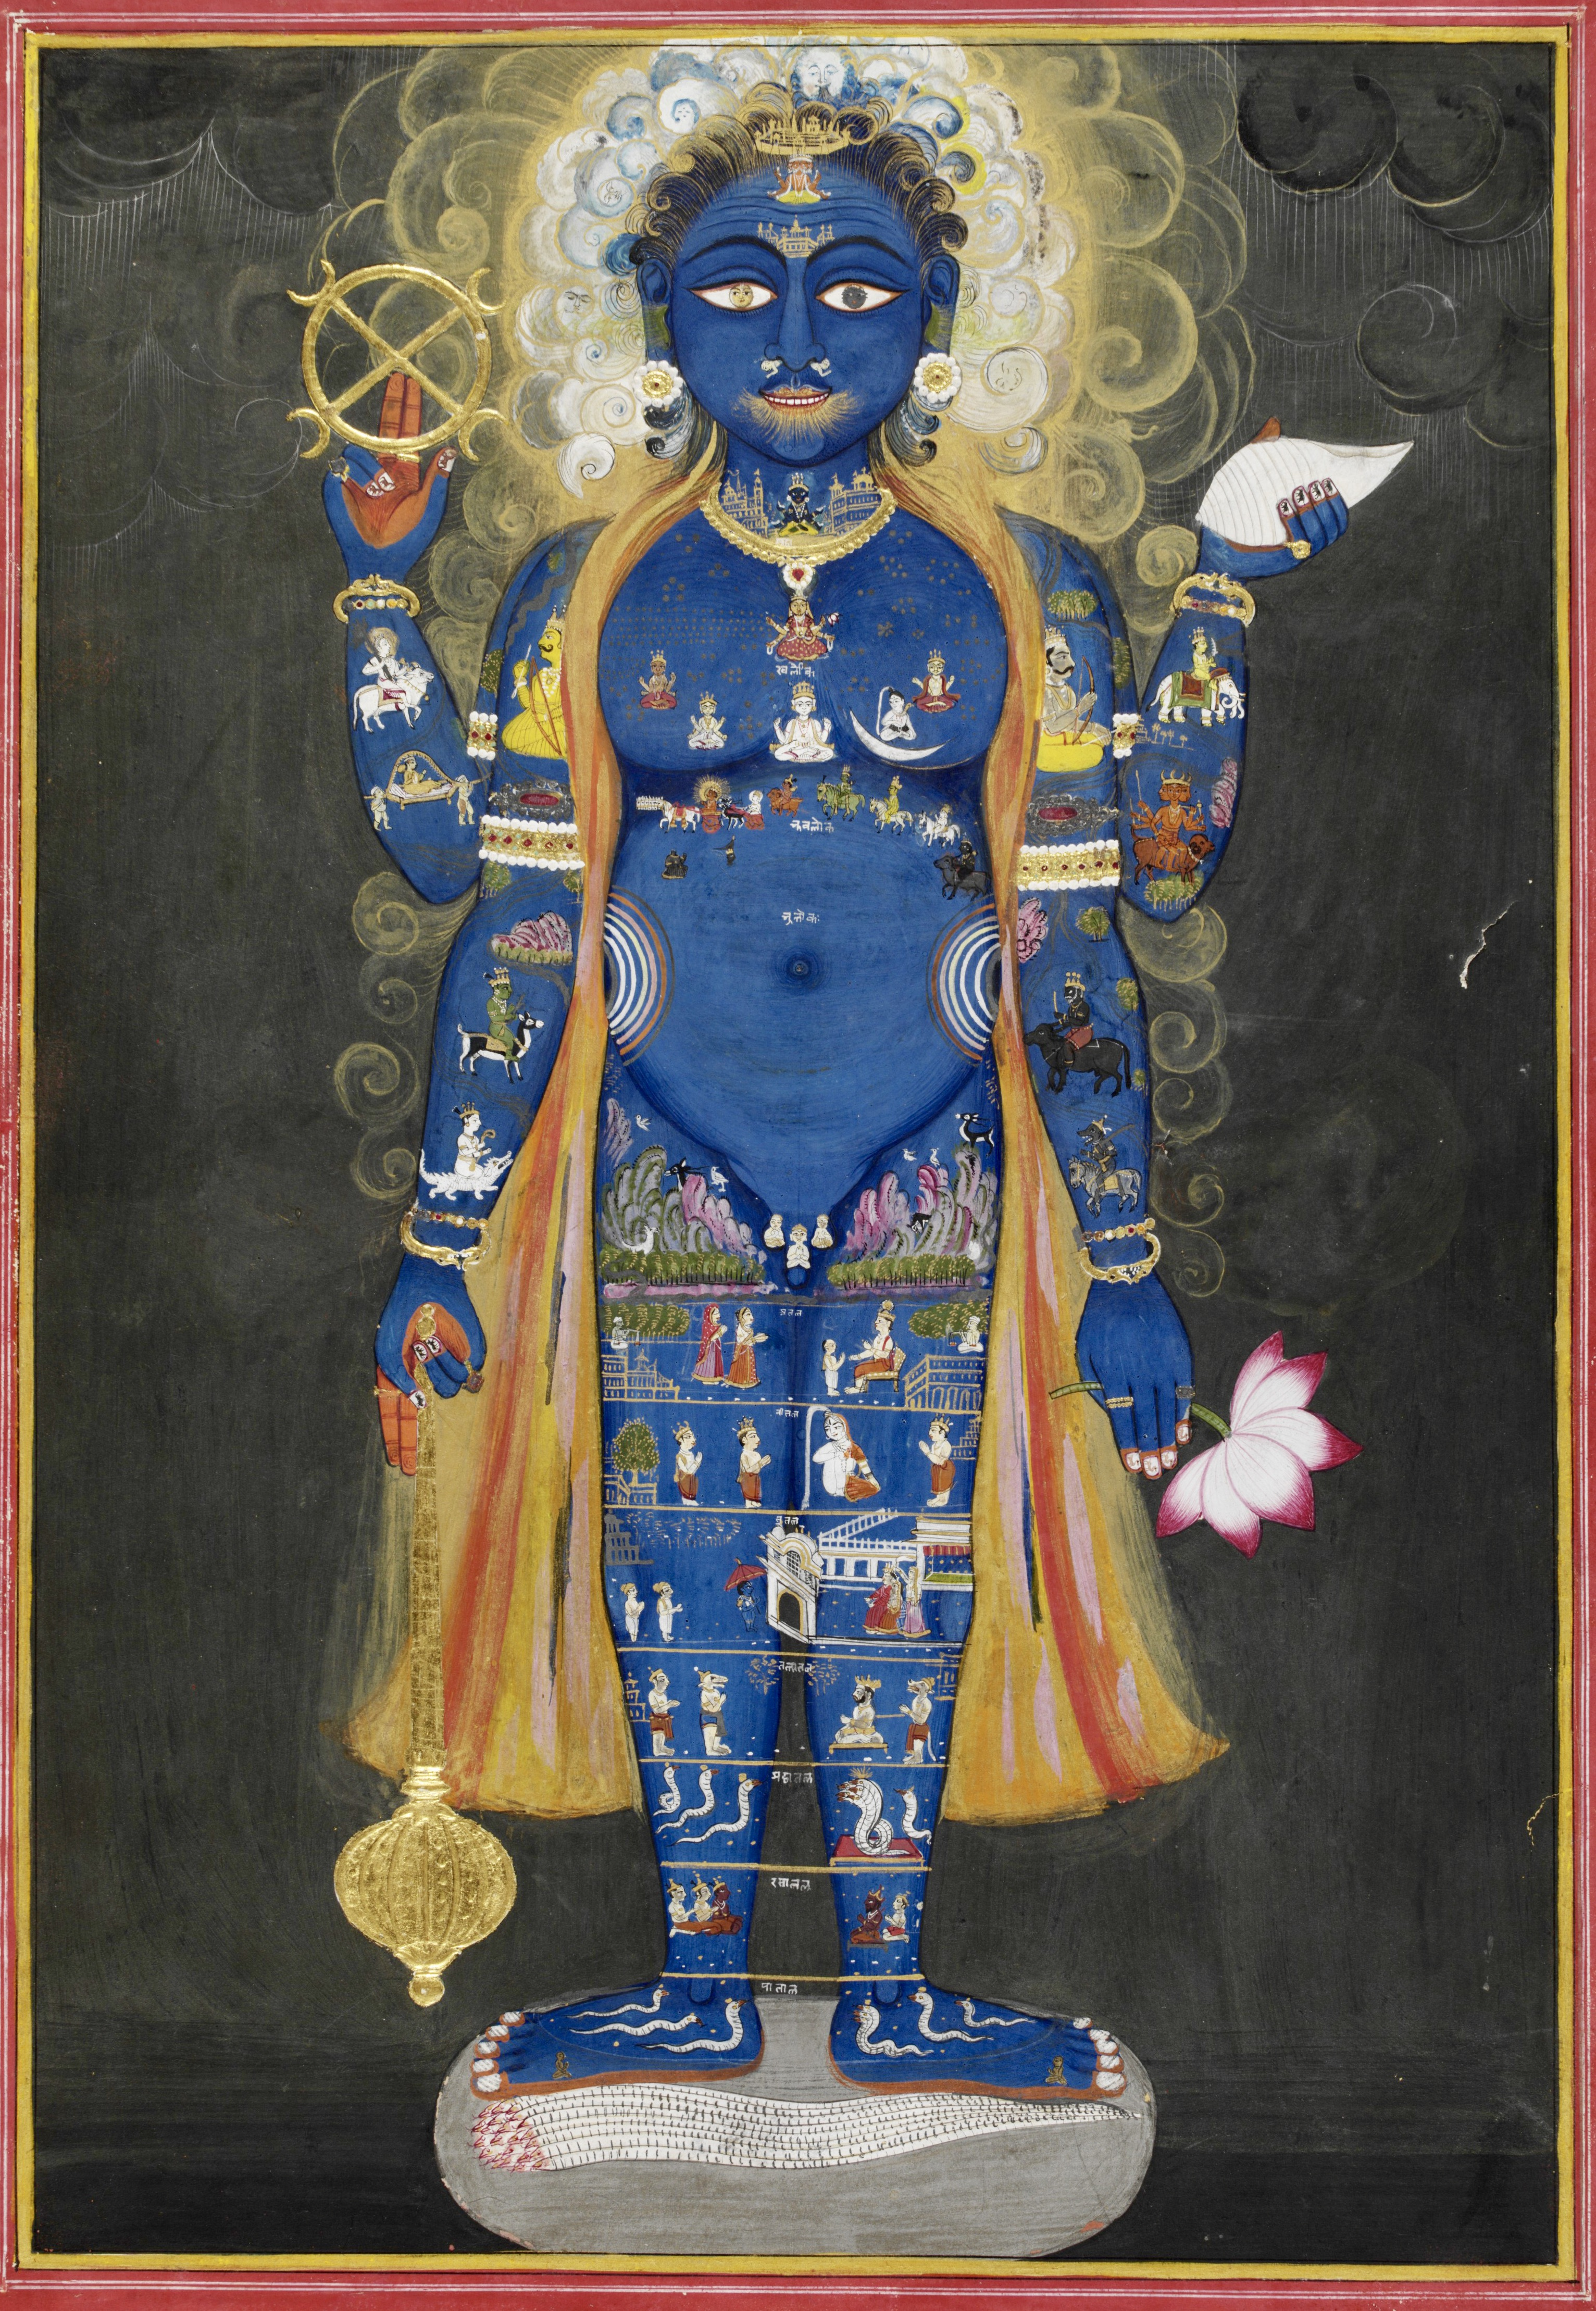
\includegraphics[width=1\textwidth]{pics/Vishnu_Vishvarupa_cropped.jpg}
	\caption{Viṣṇu Viśvarūpa, India, Rajasthan, Jaipur, ca. 1800–1820, Opaque watercolor and gold on paper, 38.5 × 28 cm, Victoria and Albert Museum, London, Given by Mrs. Gerald Clark.}
	\label{fig1}
      \end{figure}
\clearpage
  \begin{figure}[ht]
	\centering
  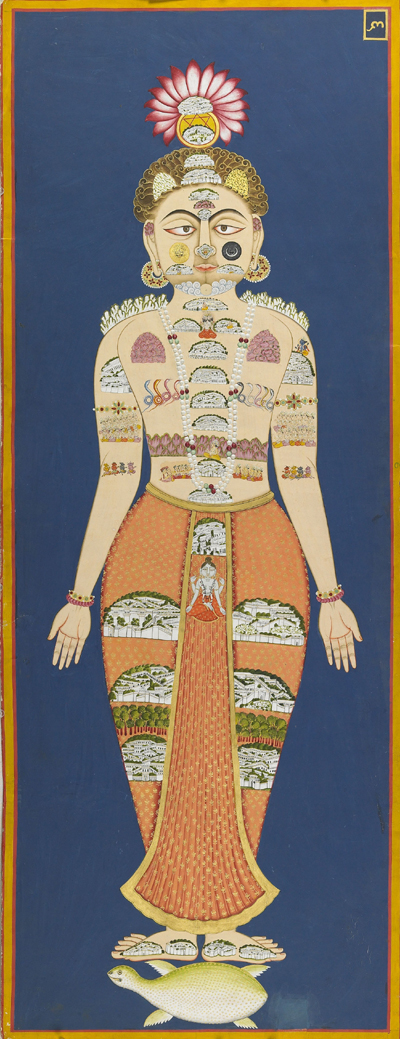
\includegraphics[width=0.5\textwidth]{pics/The_Equivalence_of_Self_and_Universe_(detail),_folio_6_from_the_Siddha_Siddhanta_Paddhati,_(Bulaki),_1824_(Samvat_1881);_122_x_46_cm._Mehrangarh_Museum_Trust..jpg}
	\caption{The Equivalence of Self and Universe (detail), folio 6 from the \textit{Siddhasiddhāntapaddhati} (Bulaki), India, Rajasthan, Jodhpur, 1824 (Samvat 1881), 122 x 46 cm, RJS 2378, Mehragarh Museum Trust.}
	\label{fig2}
      \end{figure}
      % \end{landscape}


\chapter{Bibliography}
 \label{sec:bibli}
   \clearpage
\newpage 
\thispagestyle{empty}
\quad  \addtocounter{page}{-1}

\printbibliography[heading=subbibintoc, title=Consulted Manuscripts, keyword=codex]

\printbibliography[heading=subbibintoc, title=Printed Editions, keyword=printsource]

\printbibliography[heading=subbibintoc, title=Secondary Literature, keyword=seclit]

\printbibliography[heading=subbibintoc, title=Online Sources, keyword=onlinesource]

\end{document}
